\documentclass[../report.tex]{subfiles}
\begin{document}

\onehalfspacing

\section{System Design}

\subsection{Hardware}

\subsubsection{SPI Flash}

Each Chrome book comes with 8 Mbs of non-volatile Flash memory~\cite{fw-summit}.
The memory is organized according to Figure~\ref{fig:fmap}. 
This organization is stored in a structure called the Flash Map, or fmap, and it is used by the software to read information out of Flash.
The Flash memory is connected to the CPU by the Serial Peripheral Interface (SPI).
The SPI driver handles the protocol and provides an interface for reading multiple bytes of of memory at once.

% TODO: check if there is some sort of mass info transfer, this seems really slow.
% TODO: get some sources up in hereee

\begin{figure}
  \centering
  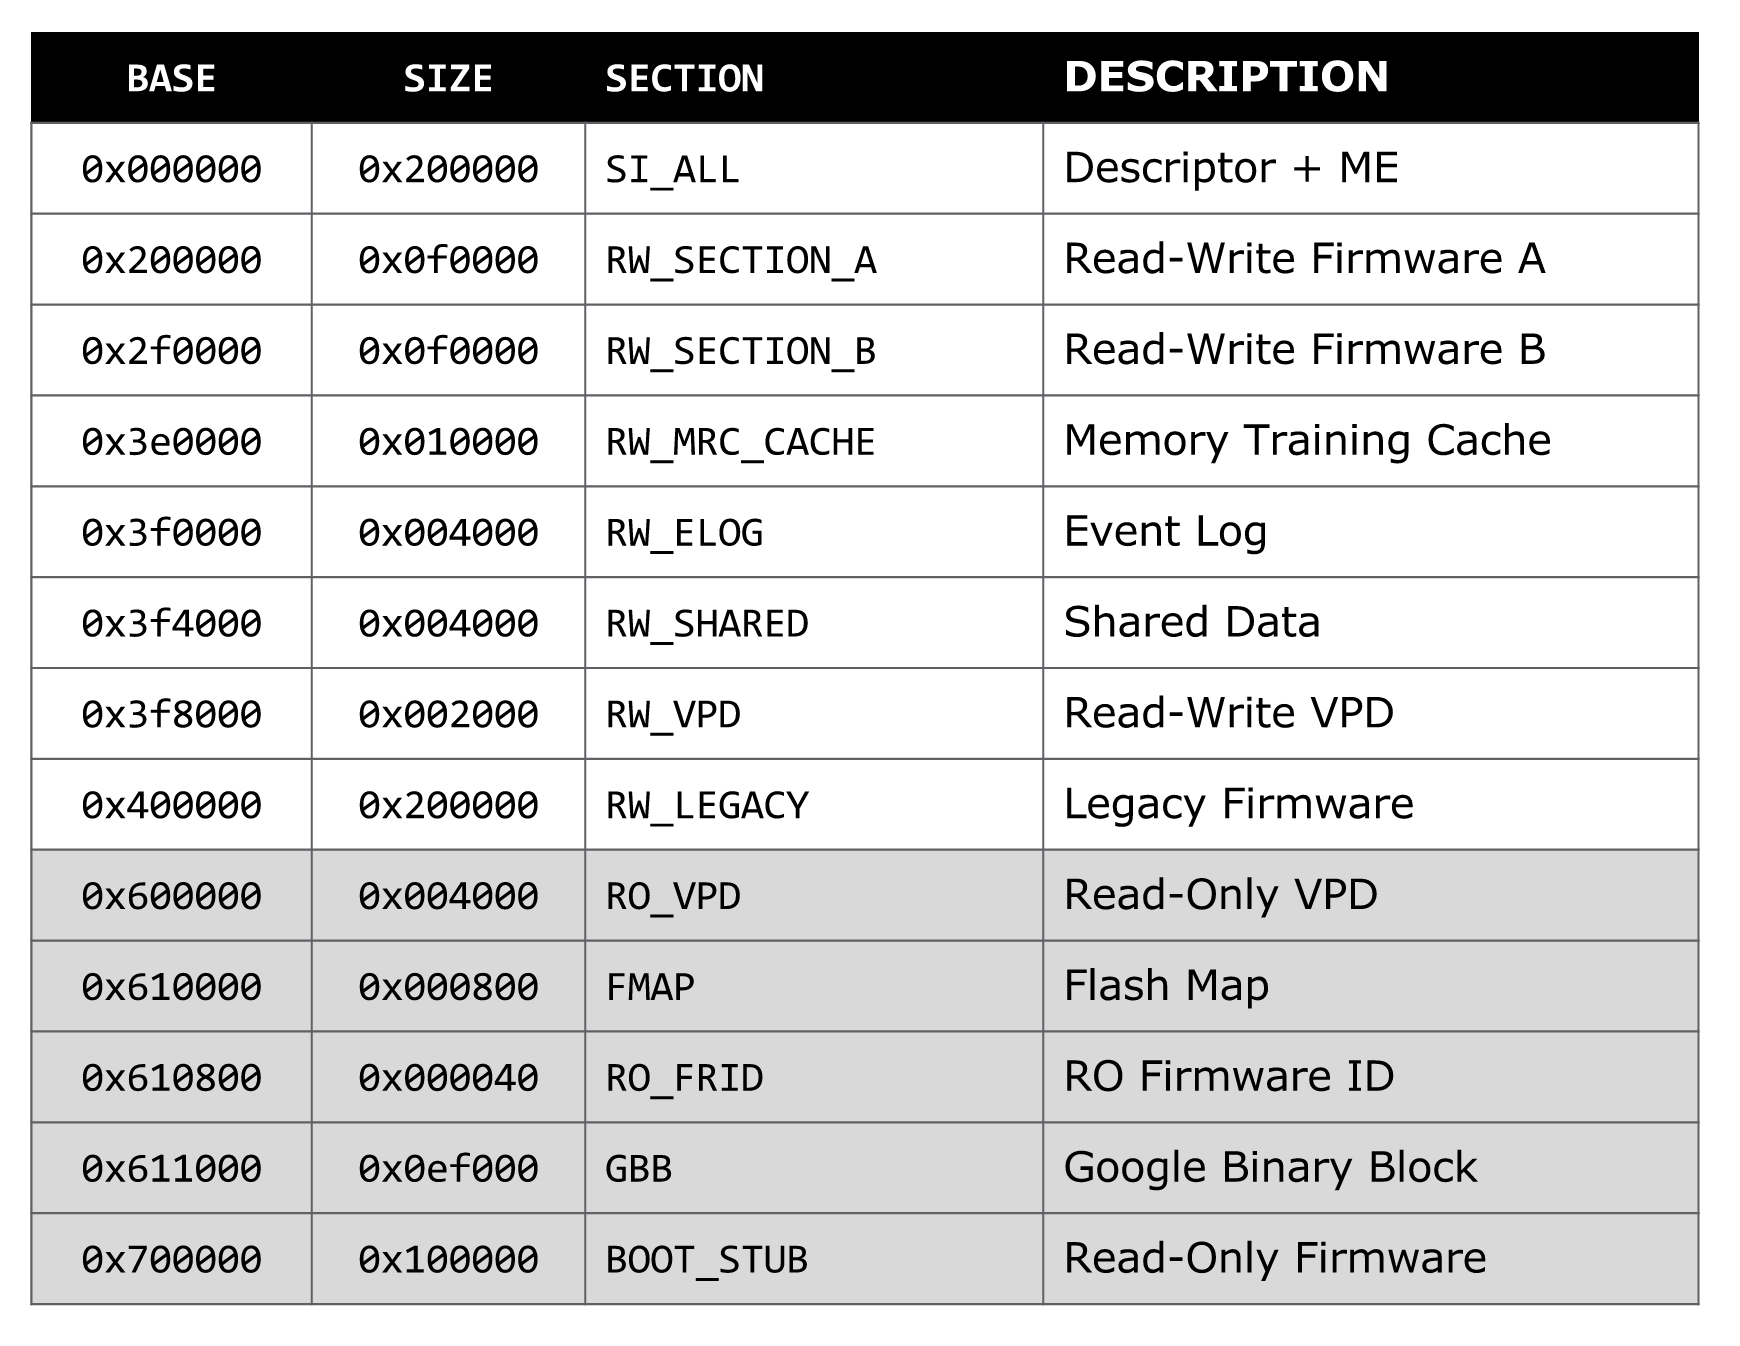
\includegraphics[width=0.8\linewidth]{fmap_locs.png}
  \caption{The Flash Map for Chrome OS's SPI Flash. The gray sections have been marked as Read Only~cite\cite{fw-summit}}
  \label{fig:fmap}
\end{figure}

The gray partitions in Figure~\ref{fig:fmap} are known as the Read-Only Flash memory.
The Read-Only memory has been set as read only by the placement of a physical screw known as the Write Protect (WP) Screw.
If the WP Screw remains in the laptop, all writes to these Flash locations will fail.
Google considers the warranty of the laptop to be voided if the screw is removed, as the laptop loses all possible security protections. 

The Read-Only memory is flashed into the laptop when the Chromebook is being built in the factory, before the Read-Only screw is added to the casing. 
The Reset Vector of the CPU points to the Read-Only flash memory, so Chrome OS is in full control of the initial software being run on the machine.
The RO Firmware contains Coreboot and Depthcharge code that drives the initialization of the hardware and the verified boot process. 
In this way the RO Flash acts as the ``Root of Trust'' for the system.
In security terms, the Verified Boot process should be secure as long as the Root of Trust holds.
Inversely, if someone removes the WP screw, none of the Verified Boot security properties will hold.


\subsubsection{TPM}

\subsubsection{External Controller}

\subsubsection{SHA}

\end{document}
